% pro and contr
\begin{frame}[t, fragile]{Pros and Cons}
\vspace{-3.5ex}
\cwpa{
    \small
    \begin{itemize}
        \item[$+$] When you have lots of equations\vspace{-1ex}
        \item[$+$] When you have a complex, but typical document \vspace{-1ex}
        \item[$+$] When you carry about device-independant view\vspace{-1ex}
        \item[$+$] When you don't want not care about the beauty, but want it\vspace{-1ex}
        \item[$+$] When you are care about the beauty wery much\vspace{-1ex}
        \item[$+$] When you hate all these humanitarian GUI programs
        % \item[$+$] When you love text files 
        % \item[``+''] When you want to impress your partner
        % yeah, I leave the commented item for you, source-code reader!
    \end{itemize}
}{
    \small
    \begin{itemize}
        \item[$-$] when you want to put something in attributary position\vspace{-1ex}
        \item[$-$] when you want to do something ``against the rules''\vspace{-1ex}
        \item[$-$] when you want to work with visual-based things (tables,...)\vspace{-1ex}
        \item[$-$] when you want to do something really simple \vspace{-1ex}
        \item[$-$] when you want to do something ``quick and dirty'' \vspace{-1ex}
    \end{itemize}
}[t]

\cprotect\skfootnote{
\verb|\item[$+$]|
}
\end{frame}

\begin{frame}{Science reseach about \LaTeX}\relax
     \begin{center}
     ``We show that LaTeX users were {\color{red}slower} than Word users <...> and produced {\color{red}more typesetting},<...>. LaTeX users, however, more often report {\color{green}enjoying using} their respective software.''          
     \end{center}

     
\skfootnote{\url{https://journals.plos.org/plosone/article?id=10.1371/journal.pone.0115069} (or in russian \url{https://habr.com/post/375109/})}
\end{frame}

\begin{frame}{Illustration}\relax
\begin{center}
     
     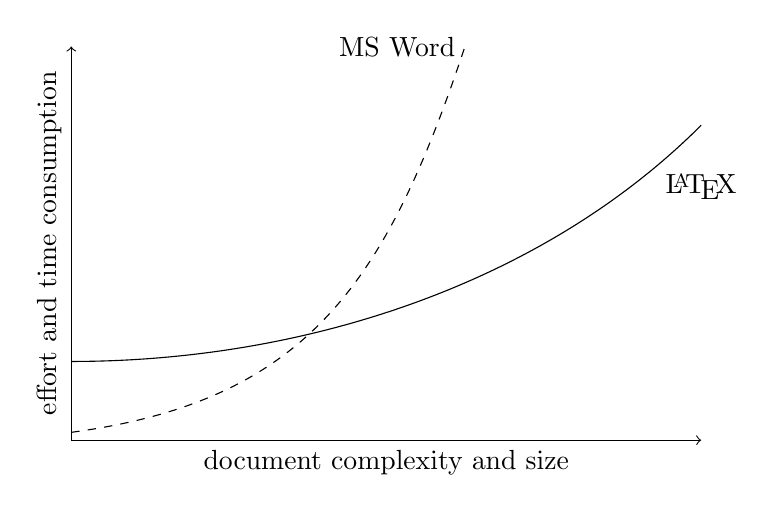
\begin{tikzpicture}[axes/.style=,important line/.style={very thick},]
        \begin{scope}[axes]
        \draw[->] (0,0) -- coordinate (x axis mid) (8,0);
    	\draw[->] (0,0) -- coordinate (y axis mid) (0,5);
    	\node[below] at (x axis mid) {document complexity and size};
    	\node[rotate=90, above] at (y axis mid) {effort and time consumption};
        \end{scope}
        \draw (0, 1)  .. controls (3,1) and (6,2) .. (8, 4) node[below=0.5cm]{\LaTeX};
        \draw[dashed] (0, 0.1) .. controls (3, 0.5) and (4,2) .. (5, 5) node[left]{MS Word};
     \end{tikzpicture}
\end{center}
     \skfootnote{based on \url{http://www.pinteric.com/miktex.html} picture\\ tikZ for plotting \url{http://www.texample.net/tikz/examples/line-plot-example/}}
\end{frame}


\begin{frame}{Common belief}\relax
    \begin{center}
        \begin{tikzpicture}
             \node[align=center] (0,0) {
             \huge \LaTeX\ is only for use\\ \huge  in academic area
             };
             \uncover<2>{\node[rotate=30, bottom color=red!50, top color=red!50] (0,0) {\Huge WRONG}};
        \end{tikzpicture}
         
    \end{center}
    \skfootnote{It was done with \tt TikZ}
\end{frame}

\begin{frame}[t]{The power of \LaTeX\ in it's templates and flexability!}\relax
\vspace{-1ex}
     Look at examples at:
     \begin{itemize}
         \item \url{https://www.latextemplates.com/}
         \item \url{https://tex.stackexchange.com/questions/158668/nice-scientific-pictures-show-off}
         \item \url{https://tex.stackexchange.com/questions/1319/showcase-of-beautiful-typography-done-in-tex-friends}
        \item $\cdots$
     \end{itemize}
     
     \vspace{-1ex}
\inclassFrag{  Please, look at these sites for two minutes  }[-1]
     
     \skfootnote{here are some more links \stExC{https://tex.stackexchange.com/questions/1362/latex-template-gallery}
     }
\end{frame}

\begin{frame}{Conclusion}\relax 

Now, in \the\year , using \LaTeX\ to write scientific articles with no math inside is more metter of joy, not productivity: MS Office took over lots of \LaTeX 's ideas.\\[2ex]

But \LaTeX\ becoming better too! because of packages, online tools and developing \LaTeX 3.

And for something as complex as this presentation you'll spend way too more time, trying to reproduce it with MS Office.
     
     \skfootnote{If you compile this presentation from source, you'll find that the year in the slide -- is the year of compilation :)}
\end{frame}


% view
\begin{frame}{What we have}
\skfootnote{\wikiC{https://en.wikibooks.org/wiki/LaTeX/Introduction}\\ \normalfont\url{http://www.texample.net/tikz/examples/tree/}}
\begin{center}
\begin{tikzpicture}[sibling distance=10em,
  every node/.style = {shape=rectangle, rounded corners,
    draw, align=center,
    top color=white, bottom color=skoltechgreen!20}]]
  \node {\TeX}
    child { node {\LaTeX}
      child { node {XeLaTeX} }
      child { node {LuaTeX} }
      } ;
\end{tikzpicture}

\end{center}
\end{frame}

\note[itemize]{
\item Start from \LaTeX
}

% LaTeX
\begin{frame}{Definitions}
\skfootnote{\normalfont\url{https://ru.wikipedia.org/wiki/LaTeX}}
\begin{columns}
\begin{column}{0.5\textwidth}
\begin{tikzpicture}[sibling distance=10em,
  every node/.style = {shape=rectangle, rounded corners,
    draw, align=center,
    top color=white, bottom color=skoltechgreen!20}]]
  \node {\TeX}
    child { node[text=red] {\LaTeX}
      child { node {XeLaTeX} }
      child { node {LuaTeX} }
      } ;
\end{tikzpicture}
\end{column}

\begin{column}{0.5\textwidth}
\small
{\csk \LaTeX} --- is the most popular set of macro-extensions (or macro package) of the computer typesetting system \TeX, which facilitates a typesetting of complex documents.

\end{column}
\end{columns}
\end{frame}

\note[itemize]{
\item What is macro 
\item macros = shortcuts 
}

% TeX
\begin{frame}{Definitions}
\skfootnote{\normalfont\url{https://en.wikipedia.org/wiki/TeX}}
\begin{columns}
\begin{column}{0.5\textwidth}
\begin{tikzpicture}[sibling distance=10em,
  every node/.style = {shape=rectangle, rounded corners,
    draw, align=center,
    top color=white, bottom color=skoltechgreen!20}]]
  \node[text=red] {\TeX}
    child { node {\LaTeX}
      child { node {XeLaTeX} }
      child { node {LuaTeX} }
      } ;
\end{tikzpicture}
\end{column}

\note{
how to pronaunce\\
Book The Art of Computer Programming \\ 
History 1978 (pdf=1993)
}

\begin{column}{0.5\textwidth}
\small
{\csk \TeX} --- is a typesetting system designed and mostly written by Donald Knuth. TeX was designed with two main goals in mind: to allow anybody to produce high-quality books using minimal effort, and to provide a system that would give exactly the same results on all computers, at any point in time

\end{column}
\end{columns}
\end{frame}

% LuaTeX and XeLaTeX
\begin{frame}{Definitions\preMagicPage}
\skfootnote{\normalfont\url{https://en.wikipedia.org/wiki/LuaTeX}, \url{https://en.wikipedia.org/wiki/XeTeX}}
\begin{columns}
\begin{column}{0.5\textwidth}
\begin{tikzpicture}[sibling distance=10em,
  every node/.style = {shape=rectangle, rounded corners,
    draw, align=center,
    top color=white, bottom color=skoltechgreen!20}]]
  \node {\TeX}
    child { node {\LaTeX}
      child { node[text=red] {XeLaTeX} }
      child { node[text=red] {LuaTeX} }
      } ;
\end{tikzpicture}
\end{column}

\begin{column}{0.5\textwidth}
\small
{\csk XeLaTeX} --- XeTeX is a \TeX typesetting engine using Unicode and supporting modern font technologies such as OpenType, Graphite and Apple Advanced Typography

{\csk LuaTeX} --- LuaTeX is a \TeX-based computer typesetting system which started as a version of pdfTeX with a Lua scripting engine embedded
\end{column}
\end{columns}
\end{frame}



\begin{frame}{Resourses\magicPage}%{Books etc}

\vspace{-3.0ex}
\begin{itemize}
    \item Knuth ``The \TeX Book'' (en, ru)
    \item L'vovsky ``Nabor i verstka v sisteme \LaTeX'' (ru)
    \item Lamport. ``\LaTeX. A Document Preparation System, User’s Guide and Reference Manual'' (en)
    \item Gratzer ``Math into \LaTeX'' (en) 
    \item Oetiker ``The Not So Short Introduction to \LaTeX'' (en, ru)
    \item \url{https://www.overleaf.com/learn}
    \item \url{https://www.latex-project.org/help/}
    \item \url{https://texfaq.org/}
\end{itemize}
\end{frame}

\note{
We will use papeeria\\
pointed about footnotes and colors!
}

\begin{frame}[fragile]{Resourses \magicPage}{Interesting links}
\cprotect\skfootnote{
\verb|\begin{description} \item[questions about \TeX]\end{description}|
}
\small
\begin{description}
    \item[questions about \TeX] \url{https://tex.stackexchange.com} \vspace{-1ex}
    \item[knowing a command of the symbol] \url{http://detexify.kirelabs.org/classify.html} \vspace{-1ex}
    \item[beauty of TikZ] \url{http://www.texample.net/tikz/examples/} \vspace{-1ex}
    \item[beauty of pictures] \url{https://tex.stackexchange.com/questions/158668/nice-scientific-pictures-show-off}\vspace{-1ex}
    \item[beauty of typesetting] \url{https://tex.stackexchange.com/questions/1319/showcase-of-beautiful-typography-done-in-tex-friends}\vspace{-1ex}
\end{description}
\end{frame}

\begin{frame}[fragile]{where to get}
\begin{enumerate}
    \item Online
    \begin{itemize}
        \item \url{http://papeeria.com}
        \item \url{https://overleaf.com}
    \end{itemize}
    \item Offline
    \begin{itemize}
        \item \LaTeX{} \url{https://www.latex-project.org/get/}
        \item package manager \verb'tlmgr'
    \end{itemize}
\end{enumerate}
     
\end{frame}






